%==============================================================================
% Sjabloon poster bachproef
%==============================================================================
% Gebaseerd op document class `a0poster' door Gerlinde Kettl en Matthias Weiser
% Aangepast voor gebruik aan HOGENT door Jens Buysse en Bert Van Vreckem

\documentclass[a0,portrait]{hogent-poster}

% Info over de opleiding
\course{Bachelorproef}
\studyprogramme{toegepaste informatica}
\academicyear{2022-2023}
\institution{Hogeschool Gent, Valentin Vaerwyckweg 1, 9000 Gent}

% Info over de bachelorproef
\title{Portals voor Quivvy Solutions: Een vergelijking van Softr, Stacker en Bubble in Web \& Mobile Toepassingen}
\subtitle{}
\author{Joeri Verhelst}
\email{joeri.verhelst@student.hogent.be}
\supervisor{Sonia Vandermeersch}
\cosupervisor{Mike Demunter (Quivvy Solutions)}

% Indien ingevuld, wordt deze informatie toegevoegd aan het einde van de
% abstract. Zet in commentaar als je dit niet wilt.
\specialisation{Mobile \& Enterprise Development}
\keywords{Low-Code, No-Code, Softwarebedrijven}
\projectrepo{https://github.com/JoeriVerhelst/JoeriVerhelst_BP}

\begin{document}

\maketitle

% \begin{abstract}
% \end{abstract}

\begin{multicols}{2} % This is how many columns your poster will be broken into, a portrait poster is generally split into 2 columns

\section{Introductie}
De zeer snelle opmars van digitalisatie zorgt ervoor dat kleine softwarebedrijven zoals 
Quivvy Solutions zorgvuldig moeten bepalen welke platformen men gebruikt om software 
zo snel mogelijk te ontwikkelen in mobile \& web toepassingen. 
Maar welke platform is nu het meest geschikt voor Quivvy Solutions waarbij het platform 
noodzakelijk moet kunnen integreren met MAKE.com en Airtable? Momenteel is er nog 
geen onderzoek gedaan over Low-Code en No-code platformen die integreren met MAKE.com 
en Airtable. Om een ruime kennis te behalen over deze platformen zal men kijken naar veiligheid, 
voordelen, nadelen en nog meer. Vervolgens heeft dit onderzoek verschillende platformen 
geanalyseerd en getest om te bepalen welke platform men aanraadt voor het softwarebedrijf.

\section{Experimenten}
Voor een grondig en gestructureerde onderzoek is er alvorens een requirements analyse 
gedaan waarbij de volgende criteria werd opgesteld;
\vspace*{1cm} % Voegt 1 cm ruimte bovenaan toe
\begin{itemize}
    \item Snelheid van het platform
    \item Herstelbeheer
    \item Veiligheid
    \item Snelheid van applicatieontwikkeling
    \item Integratiemogelijkheden
    \item Platformflexibiliteit (bv. high-code kunnen implementeren)
    \item Schaalbaarheid
    \item Gebruiksvriendelijkheid
    \item Integratie met AirTable en/of MAKE.com
    \item Kostprijs
    \item Updatebeleid
\end{itemize}
\vspace*{1cm} % Voegt 1 cm ruimte onderaan toe
Na de vereisten werd er dan een 5 aantal alternatieven 
platformen gekozen en onderzocht aan de hand van de criteria. 
Vervolgens werd er dan ook één alternatief gekozen voor verder onderzoek. 
Daarna nam er een vergelijkende analyse plaats die de drie platformen; Softr, Stacker en Bubble 
analyseerde via de criteria. De informatie van de platformen werden gehaald uit online bronnen; 
websites van bedrijven, officiële website, blogs van expertises in het vakgebied. Om een zekere 
beslissing te nemen nam er een Proof of Concept plaats waarbij een programmeur verschillende 
criteria had getest. De applicatie die de programmeur moest maken bestond uit een feedback 
formulier waarbij de data bewaard werd in Airtable en via MAKE.com een e-mail werd verstuurd 
naar de gebruiker. Daarbij moest het ook een scherm bevatten met een lijst  van alle feedback. 
Vervolgens namen ook 3 niet-programmeurs, die geen IT-kennis hebben, deel aan het POC. 
Voor hun was het iets anders dat ze moesten maken, namelijk een TODO app. 
Bij de niet-programmeurs was het dan ook vooral testen op de gebruiksvriendelijkheid

% \section{Sectie met figuur}

% De {\LaTeX} figure-omgeving bepaalt zelf waar een afbeelding komt en dat is meestal niet op de plek in de tekst waar de figure-omgeving gedefinieerd wordt. Als je wilt forceren dat afbeeldingen toch in de flow van de tekst blijven, dan kan je dat zoals hieronder:

% \begin{center}
%   \captionsetup{type=figure}
%   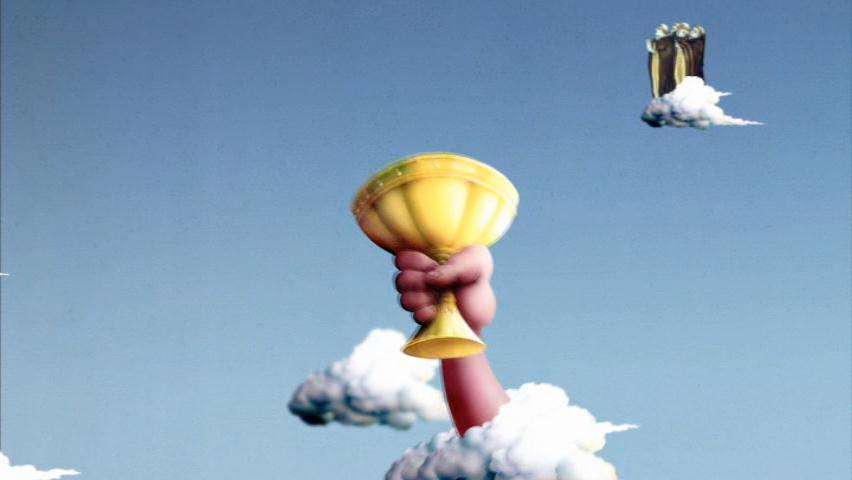
\includegraphics[width=1.0\linewidth]{grail}
%   \captionof{figure}{He hasn't got shit all over him. The nose? Where'd you get the coconuts? What do you mean? We shall say `Ni' again to you, if you do not appease us}
% \end{center}

% Let er wel op dat dit tot problemen met bladschikking kan leiden.
\section{Resultaten}
Uit het onderzoek is er heel wat interessante data naar boven gekomen bij elk platform. 
Als we eens een kijkje nemen naar Bubble kreeg dit platform een 3.7/5 op de ervaring van de gebruikers in de Proof Of Concept. 
Dit omdat het implementeren van logica niet eenvoudig was. Daarnaast kost het platform tussen de 29 en 349 dollar per maand. 
Het interessante aan Bubble is dat er een community marketplace is voor templates en plugins. Het is ook zo dat Bubble meer schaalbaar 
is dan Softr omdat het niet gelimiteerd is op het aantal gebruikers van je app of website. Dit is niet zo bij Softr want hier is het namelijk 
afhankelijk van je abonnement. Softr scoort op ervaring een 4.3/5, wat het hoogste is van allemaal. Voor Softr betaal je tussen de 59 en 
1.000 dollar per maand. Als laatste is er Stacker die een beoordeling van 3.3/5 heeft voor de ervaring van gebruikers. 
De reden hiervoor is omdat het zeer beperkt is op vlak van platformflexibiliteit. Maar het kan ook niet integreren met MAKE.com. 
Dit platform heeft een kostprijs tussen 79 en 349 dollar per maand.
\section{Conclusies}
Men kan concluderen dat Bubble aangeraden wordt aan Quivvy Solutions. 
Door de ruime methodologie konden we deze conclusie neertoetsen op bepaalde punten. 
Het is namelijk zo dat het noodzakelijk is voor het bedrijf dat het kan integreren met Airtable en MAKE.com, 
wat Bubble kan. Vervolgens is de platformflexibiliteit en de mogelijkheid hebben om verschillende databases te 
gebruiken superieur tegenover Softr en Stacker. Er werd ook opgemerkt dat Bubble interessant is voor lange termijn en 
grote bedrijven door de goede schaalbaarheid. De kostprijs van Bubble is minder duur dan de twee andere platformen, 
wat ideaal is voor kleine softwarebedrijven. Vervolgens wil je als bedrijf ook dat het constant updates heeft. Bubble is 
hier dan ook beter in dan de andere. Het heeft namelijk constant updates die zeer transparant zijn naar hun gebruikers 
toe. Het enigste waar Bubble niet beter is, is op het vlak van gebruiksvriendelijkheid en snelheid van applicatieontwikkeling.

\section{Toekomstig onderzoek}
 Helaas werden deze drie platformen niet getest op het maken van uitgebreide complexe apps en websites. Daarbij bestond het POC maar vier participanten.
Het zou interessant zijn om deze platformen te testen op het maken van complexe apps en websites. Daarbij zou het ook interessant zijn om meer participanten te hebben.

\end{multicols}
\end{document}